\documentclass[11pt,letterpaper,landscape]{article}

% Packages
\usepackage[margin=0.5in,landscape]{geometry}
\usepackage{tikz}
\usepackage{xcolor}
\usepackage{hyperref}
\usepackage{fancyhdr}
\usepackage{graphicx}
\usepackage{float}
\usepackage{fontenc}

% TikZ libraries
\usetikzlibrary{shapes.geometric, arrows.meta, positioning, fit, backgrounds, calc, decorations.markings, shadows, patterns}

% Colors - NOAA/AWS themed
\definecolor{noaablue}{HTML}{003087}
\definecolor{noaalight}{HTML}{4A90D9}
\definecolor{awsorange}{HTML}{FF9900}
\definecolor{awsdark}{HTML}{232F3E}
\definecolor{vpcgreen}{HTML}{1B660F}
\definecolor{securityred}{HTML}{CC2936}
\definecolor{neptunepurple}{HTML}{6B48FF}
\definecolor{opensearchblue}{HTML}{005EB8}
\definecolor{agentcoregold}{HTML}{D4A017}
\definecolor{bastiontan}{HTML}{C4A35A}
\definecolor{lightgray}{HTML}{F5F5F5}
\definecolor{cacgreen}{HTML}{2E7D32}

% Header/Footer
\pagestyle{fancy}
\fancyhf{}
\fancyhead[L]{\small\textcolor{noaablue}{NOAA/NWS/NCEP/EMC --- CAT Unit}}
\fancyhead[R]{\small\textcolor{noaablue}{Kiro IDE Connectivity Architecture}}
\fancyfoot[C]{\small Department of Commerce // National Oceanic and Atmospheric Administration}
\renewcommand{\headrulewidth}{0.4pt}

\hypersetup{colorlinks=true, linkcolor=noaablue, urlcolor=noaalight}

\begin{document}
\thispagestyle{fancy}

\begin{center}
{\Large\textbf{\textcolor{noaablue}{Kiro IDE --- CAC Authentication \& EC2 Connectivity}}}\\[0.1cm]
{\small May 2026}
\end{center}

\vspace{0.1cm}

\begin{figure}[H]
\centering
\resizebox{\textwidth}{!}{%
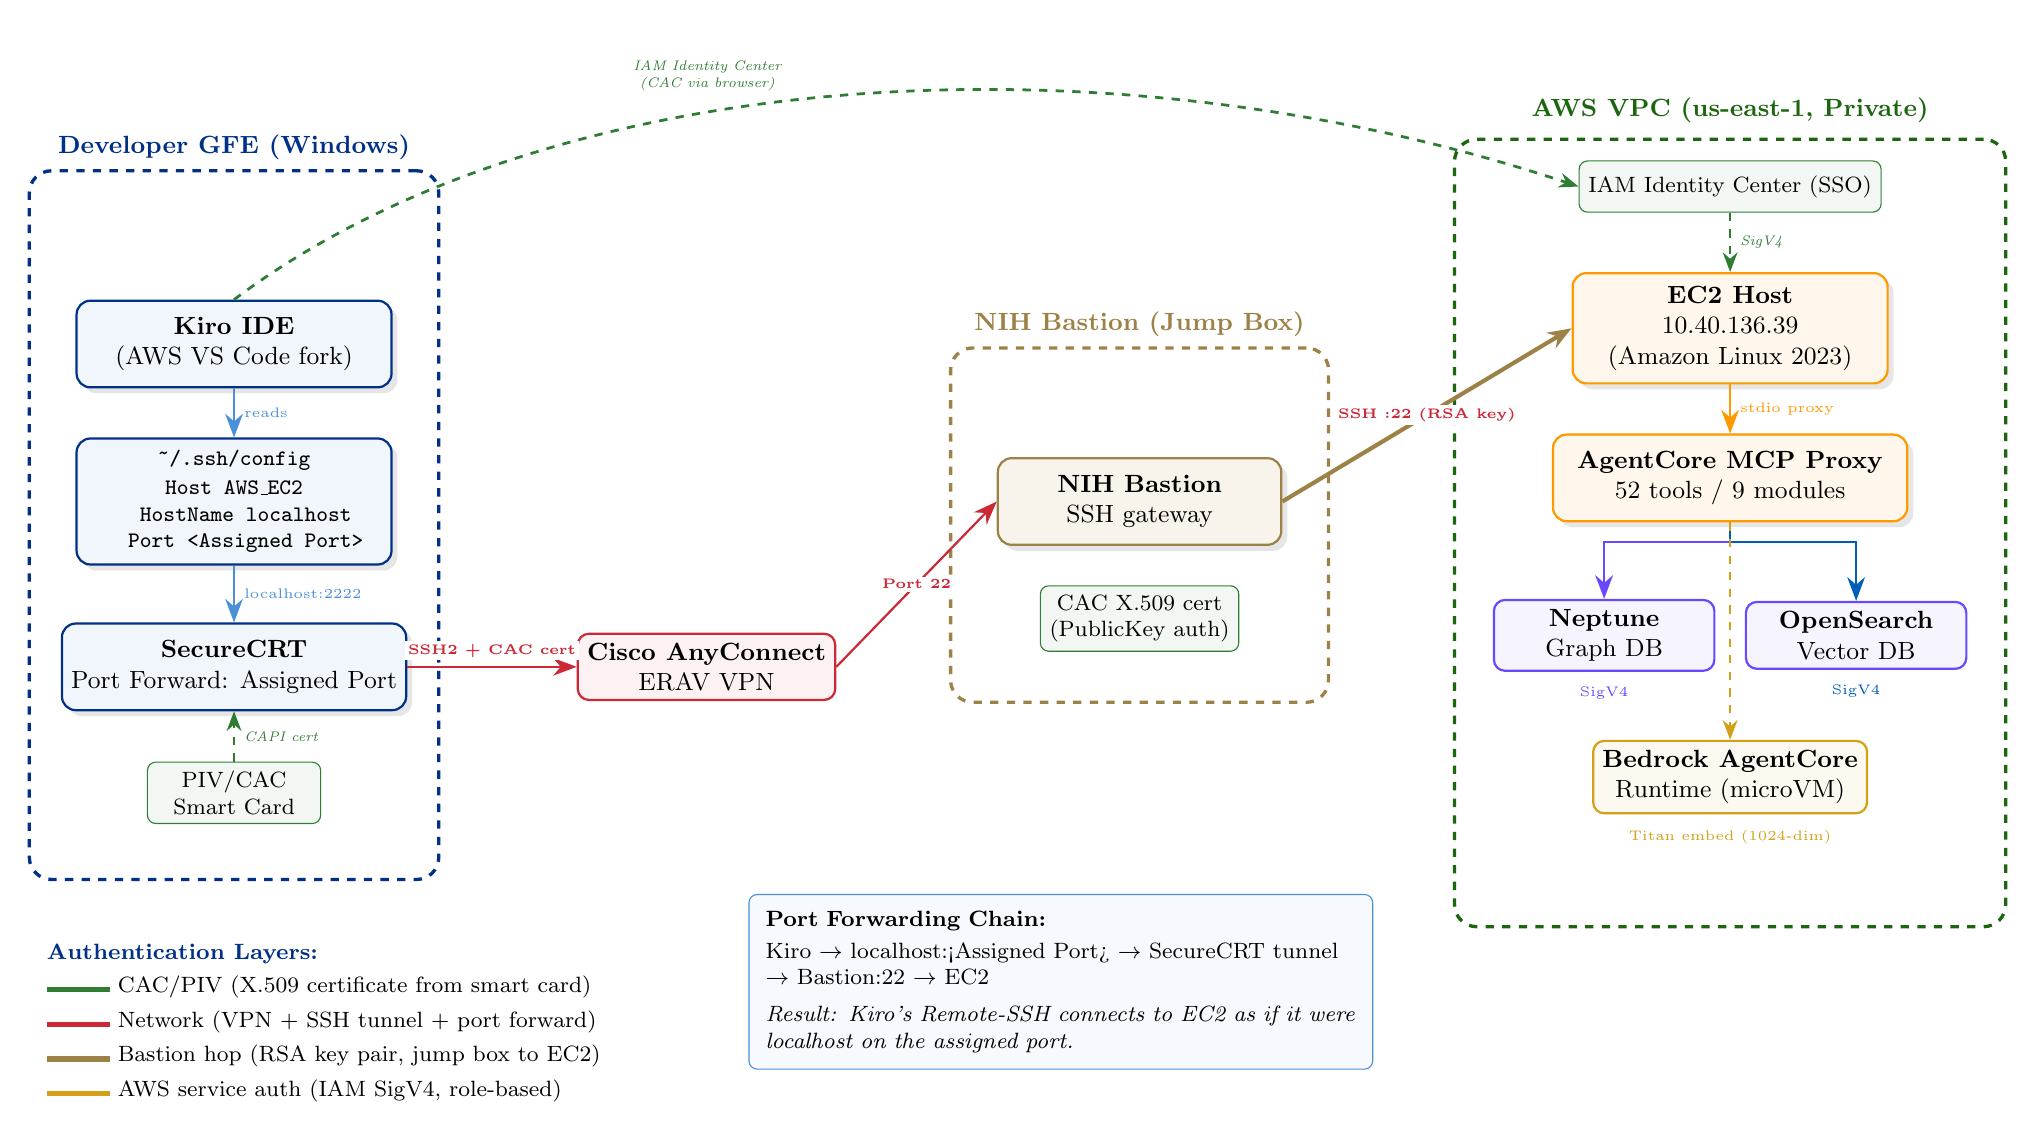
\begin{tikzpicture}[
    every node/.style={font=\small},
    % Box styles
    gfebox/.style={rectangle, draw=noaablue, fill=noaalight!8, rounded corners=5pt,
                   minimum width=4cm, minimum height=1.1cm, align=center, thick,
                   drop shadow={opacity=0.2}},
    bastionbox/.style={rectangle, draw=bastiontan!80!black, fill=bastiontan!12,
                       rounded corners=5pt, minimum width=3.6cm, minimum height=1.1cm,
                       align=center, thick, drop shadow={opacity=0.2}},
    ec2box/.style={rectangle, draw=awsorange, fill=awsorange!8, rounded corners=5pt,
                   minimum width=4cm, minimum height=1.1cm, align=center, thick,
                   drop shadow={opacity=0.2}},
    servicebox/.style={rectangle, draw=neptunepurple, fill=neptunepurple!6,
                       rounded corners=4pt, minimum width=2.8cm, minimum height=0.85cm,
                       align=center, thick},
    authbox/.style={rectangle, draw=cacgreen, fill=cacgreen!6, rounded corners=3pt,
                    minimum width=2.2cm, minimum height=0.65cm, align=center,
                    font=\footnotesize},
    vpnbox/.style={rectangle, draw=securityred, fill=securityred!6, rounded corners=4pt,
                   minimum width=3.2cm, minimum height=0.75cm, align=center, thick},
    arrow/.style={-{Stealth[length=3mm]}, thick},
    dashedarrow/.style={-{Stealth[length=2.5mm]}, thick, dashed},
    authlabel/.style={font=\tiny\itshape, text=cacgreen, align=center},
    portlabel/.style={font=\tiny\bfseries, text=securityred, fill=white, inner sep=1pt},
    zone/.style={rectangle, draw=#1, very thick, dashed, rounded corners=8pt}
]

% =====================================================================
% ZONE 1: Developer GFE (left)
% =====================================================================
\node[zone=noaablue, minimum width=5.2cm, minimum height=9cm, inner sep=14pt,
      label={[font=\small\bfseries, text=noaablue]above:Developer GFE (Windows)}]
      (gfezone) at (0, 0) {};

\node[gfebox] (kiro) at (0, 2.3) {\textbf{Kiro IDE}\\(AWS VS Code fork)};

\node[gfebox, minimum height=1.6cm, font=\footnotesize] (sshconfig) at (0, 0.3) {%
    \texttt{\textasciitilde/.ssh/config}\\[1pt]
    \texttt{Host AWS\_EC2}\\
    \texttt{~~HostName localhost}\\
    \texttt{~~Port <Assigned Port>}
};

\node[gfebox] (securecrt) at (0, -1.8) {\textbf{SecureCRT}\\Port Forward: Assigned Port};

\node[authbox] (cac) at (0, -3.4) {PIV/CAC\\Smart Card};

% Internal GFE connections
\draw[arrow, noaalight] (kiro) -- (sshconfig) node[midway, right, font=\tiny] {reads};
\draw[arrow, noaalight] (sshconfig) -- (securecrt) node[midway, right, font=\tiny] {localhost:2222};
\draw[dashedarrow, cacgreen] (cac) -- (securecrt) node[midway, right, authlabel] {CAPI cert};

% =====================================================================
% ZONE 2: VPN (between GFE and Bastion)
% =====================================================================
\node[vpnbox] (vpn) at (6, -1.8) {\textbf{Cisco AnyConnect}\\ERAV VPN};

\draw[arrow, securityred] (securecrt.east) -- (vpn.west)
    node[midway, portlabel, above=2pt] {SSH2 + CAC cert};

% =====================================================================
% ZONE 3: NIH Bastion / Jump Box
% =====================================================================
\node[zone=bastiontan!80!black, minimum width=4.8cm, minimum height=4.5cm, inner sep=18pt,
      label={[font=\small\bfseries, text=bastiontan!80!black]above:NIH Bastion (Jump Box)}]
      (bastionzone) at (11.5, 0) {};

\node[bastionbox] (bastion) at (11.5, 0.3) {\textbf{NIH Bastion}\\SSH gateway};

\node[authbox, below=0.5cm of bastion] (bastionauth) {CAC X.509 cert\\(PublicKey auth)};

% VPN to bastion (straight right)
\draw[arrow, securityred] (vpn.east) -- (bastion.west)
    node[midway, portlabel] {Port 22};

% =====================================================================
% ZONE 4: AWS VPC (right side)
% =====================================================================
\node[zone=vpcgreen, minimum width=7cm, minimum height=10cm, inner sep=18pt,
      label={[font=\small\bfseries, text=vpcgreen, yshift=2pt]above:AWS VPC (us-east-1, Private)}]
      (vpczone) at (19, -0.1) {};

% EC2 Host
\node[ec2box, minimum height=1.4cm] (ec2) at (19, 2.5) {\textbf{EC2 Host}\\10.40.136.39\\(Amazon Linux 2023)};

% MCP Server
\node[ec2box, minimum width=4.5cm, minimum height=1.1cm] (mcp) at (19, 0.6) {%
    \textbf{AgentCore MCP Proxy}\\
    52 tools / 9 modules
};

% Data stores (balanced: 3 equal gaps within VPC width of 7cm centered at x=19)
% VPC inner left edge ~15.5, inner right edge ~22.5 → usable width ~7cm
% Each box is 2.8cm wide. 3 gaps share remaining space: (7 - 2*2.8)/3 = 0.47cm
% Centers: left box at 15.5 + 0.47 + 1.4 = 17.37, right at 22.5 - 0.47 - 1.4 = 20.63
\node[servicebox] (neptune) at (17.4, -1.4) {\textbf{Neptune}\\Graph DB};
\node[servicebox] (opensearch) at (20.6, -1.4) {\textbf{OpenSearch}\\Vector DB};

% Bedrock (centered below data stores)
\node[servicebox, draw=agentcoregold, fill=agentcoregold!6] (bedrock) at (19, -3.2) {%
    \textbf{Bedrock AgentCore}\\
    Runtime (microVM)
};

% Internal VPC connections
\draw[arrow, awsorange] (ec2) -- (mcp) node[midway, right, font=\tiny] {stdio proxy};
\draw[arrow, neptunepurple] (mcp.south) -- ++(0,-0.25) -| (neptune.north);
\draw[arrow, opensearchblue] (mcp.south) -- ++(0,-0.25) -| (opensearch.north);
\node[font=\tiny, text=neptunepurple, below=2pt of neptune.south] {SigV4};
\node[font=\tiny, text=opensearchblue, below=2pt of opensearch.south] {SigV4};
% Titan embed arrow goes straight down from Bedrock to below it (annotation below Bedrock box)
\draw[dashedarrow, agentcoregold] (mcp.south) -- (bedrock.north);
\node[font=\tiny, text=agentcoregold, below=2pt of bedrock.south] {Titan embed (1024-dim)};

% =====================================================================
% IAM Auth (top right, in the freed title space)
% =====================================================================
\node[authbox, minimum width=2.8cm] (iam) at (19, 4.3) {IAM Identity Center (SSO)};

% IAM to EC2
\draw[dashedarrow, cacgreen] (iam.south) -- (ec2.north)
    node[midway, right, font=\tiny\itshape, text=cacgreen] {SigV4};

% Kiro to IAM (curved over the top)
\draw[dashedarrow, cacgreen, line width=1pt] (kiro.north) .. controls +(4,3) and +(-6,2) .. (iam.west)
    node[pos=0.4, above=4pt, authlabel] {IAM Identity Center\\(CAC via browser)};

% =====================================================================
% CROSS-ZONE ARROWS
% =====================================================================

% Bastion to EC2 (straight right)
\draw[arrow, bastiontan!80!black, line width=1.5pt] (bastion.east) -- (ec2.west)
    node[midway, portlabel] {SSH :22 (RSA key)};

% =====================================================================
% LEGEND (bottom left)
% =====================================================================
\node[font=\footnotesize\bfseries, text=noaablue, anchor=north west] at (-2.5, -5.2) {Authentication Layers:};

\node[anchor=north west, font=\footnotesize, align=left] at (-2.5, -5.6) {%
    \textcolor{cacgreen}{\rule{0.8cm}{2pt}} CAC/PIV (X.509 certificate from smart card)\\[3pt]
    \textcolor{securityred}{\rule{0.8cm}{2pt}} Network (VPN + SSH tunnel + port forward)\\[3pt]
    \textcolor{bastiontan!80!black}{\rule{0.8cm}{2pt}} Bastion hop (RSA key pair, jump box to EC2)\\[3pt]
    \textcolor{agentcoregold}{\rule{0.8cm}{2pt}} AWS service auth (IAM SigV4, role-based)
};

% =====================================================================
% Port forwarding annotation — wider text width to prevent wrapping
\node[rectangle, draw=noaalight, fill=noaalight!5, rounded corners=3pt,
      font=\footnotesize, align=left, text width=7.5cm, inner sep=6pt]
      at (10.5, -5.8) {%
    \textbf{Port Forwarding Chain:}\\[2pt]
    Kiro $\rightarrow$ localhost:<Assigned Port> $\rightarrow$ SecureCRT tunnel $\rightarrow$ Bastion:22 $\rightarrow$ EC2\\[4pt]
    \textit{Result: Kiro's Remote-SSH connects to EC2 as if it were localhost on the assigned port.}
};

\end{tikzpicture}
}% end resizebox
\caption{End-to-end connectivity: Kiro IDE on GFE laptop through CAC-authenticated bastion hop to AWS EC2 and MCP infrastructure}
\end{figure}

\end{document}
